\documentclass[tikz,border=2pt,11pt]{standalone}
\usetikzlibrary{arrows.meta}
\usetikzlibrary{positioning}
\usepackage{amsmath}
\usepackage{amssymb}
\usepackage{xcolor}
\usepackage{tikz}
\newcommand{\DoNotLoadEpstopdf}{}
\newcommand{\R}{\mathbb R}
\newcommand{\C}{\mathbb C}
\newcommand{\PP}{\mathbb P}
\newcommand{\Z}{\mathbb Z}
\newcommand{\cO}{\mathcal O}
\newcommand{\dd}{\mathrm d}
\newcommand{\id}{\mathrm{id}}
\DeclareMathOperator{\Ham}{Ham}
\DeclareMathOperator{\vol}{vol}
\DeclareMathOperator{\Bl}{Bl}
\DeclareMathOperator{\Int}{int}
\DeclareMathOperator{\supp}{supp}
\DeclareMathOperator{\pr}{pr}
\newcommand{\sq}{\mathbin{\sqcup}}
\newcommand{\eps}{\varepsilon}
\newcommand{\pair}[2]{\langle #1,#2\rangle}
\newcommand{\norm}[1]{\left\lVert #1\right\rVert}
\begin{document}
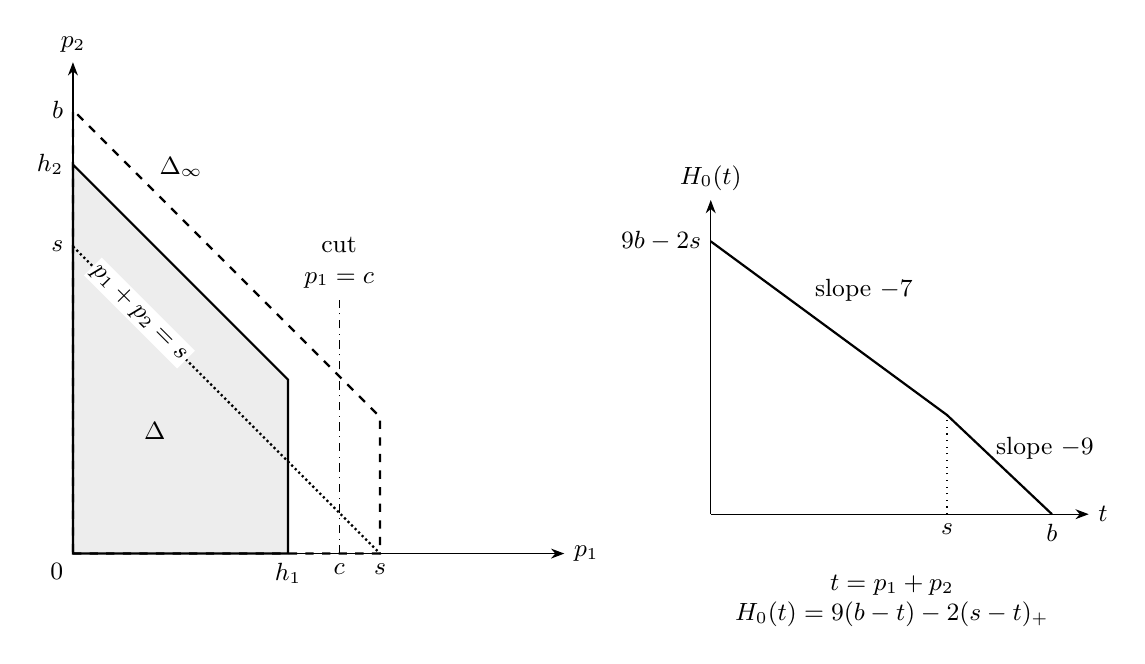
\begin{tikzpicture}[font=\small,>=Stealth]
 \begin{scope}[x=13cm,y=13cm]
  \fill[black!7] (0,0)--(.21,0)--(.21,.17)--(0,.38)--cycle;
  \draw[dashed,thick] (0,0)--(.3,0)--(.3,.133333)--(0,.433333)--cycle;
  \draw[thick] (0,0)--(.21,0)--(.21,.17)--(0,.38)--cycle;
  \draw[densely dotted,thick] (0,.3)--(.3,0);
  \draw[dash dot] (.26,0)--(.26,.25)
    node[above,align=center] {cut\\\(p_1=c\)};
  \draw[->] (0,0)--(.48,0) node[right] {\(p_1\)};
  \draw[->] (0,0)--(0,.48) node[above] {\(p_2\)};
  \node[below left] at (0,0) {\(0\)};
  \node[left] at (0,.433333) {\(b\)};
  \node[left] at (0,.38) {\(h_2\)};
  \node[left] at (0,.3) {\(s\)};
  \node[below] at (.21,0) {\(h_1\)};
  \node[below] at (.26,0) {\(c\)};
  \node[below] at (.3,0) {\(s\)};
  \node at (.08,.12) {\(\Delta\)};
  \node[above right] at (.075,.358333) {\(\Delta_\infty\)};
  \node[rotate=-45,fill=white,inner sep=1pt] at (.065,.235)
    {\(p_1+p_2=s\)};
 \end{scope}
 \begin{scope}[shift={(8.1cm,.5cm)},x=10cm,y=1.05cm]
  \draw[->] (0,0)--(.48,0) node[right] {\(t\)};
  \draw[->] (0,0)--(0,3.8) node[above] {\(H_0(t)\)};
  \draw[thick] (0,3.3)--(.3,1.2)--(.433333,0);
  \draw[dotted] (.3,0)--(.3,1.2);
  \node[left] at (0,3.3) {\(9b-2s\)};
  \node[below] at (.3,0) {\(s\)};
  \node[below] at (.433333,0) {\(b\)};
  \node[above right] at (.12,2.46) {slope \(-7\)};
  \node[right] at (.35,.8) {slope \(-9\)};
  \node[align=center] at (.23,-1.05)
    {\(t=p_1+p_2\)\\
     \(H_0(t)=9(b-t)-2(s-t)_+\)};
 \end{scope}
\end{tikzpicture}
\end{document}
